\subsection*{Introduction}

The problem consists of a dataset containing significant wave-heights recorded 14 times a month during several winter months in the north Atlantic. This is could for example be used to predict the probability of high waves in the north atlantic to warn oil platforms. One can estimate the extreme value of this dataset by assuming that the data has a \textit{Gumpel Distribution} with distribution function
\[ F(x; \mu, \beta)=\exp\left(-\exp\left(-\frac{x-\mu}{\beta}\right)\right), \quad x\in\mathbb{R}, \]
where $\mu\in\mathbb{R}$ and $\beta>0$. The paramaters of this distribution for an arbitrary dataset was estimated using the matlab function \texttt{est\_gumbel.m}. \\

During a 100 year interval, one can calculate a estimate of the likelihood of an 100--year return period event. It is a statistical measurement typically based on historic data denoting the average recurrence interval over an extended period of time. The analysis assumes that the probability does not vary in time and is independant of past events. \\

The expected 100-year return value of the data gives the largest expected wave-height during a 100-year period. The $T$:th return value is denoted by $F^{-1}(1-1/T;\mu,\beta)$. Since the data has been observed during 14 times a month and assuming we have three winter months during a year, $T$ is $T=3\cdot14\cdot100$. The investigated dataset is shown below in figure \ref{fig:waves}. \\

\begin{figure}[H]
\centering
	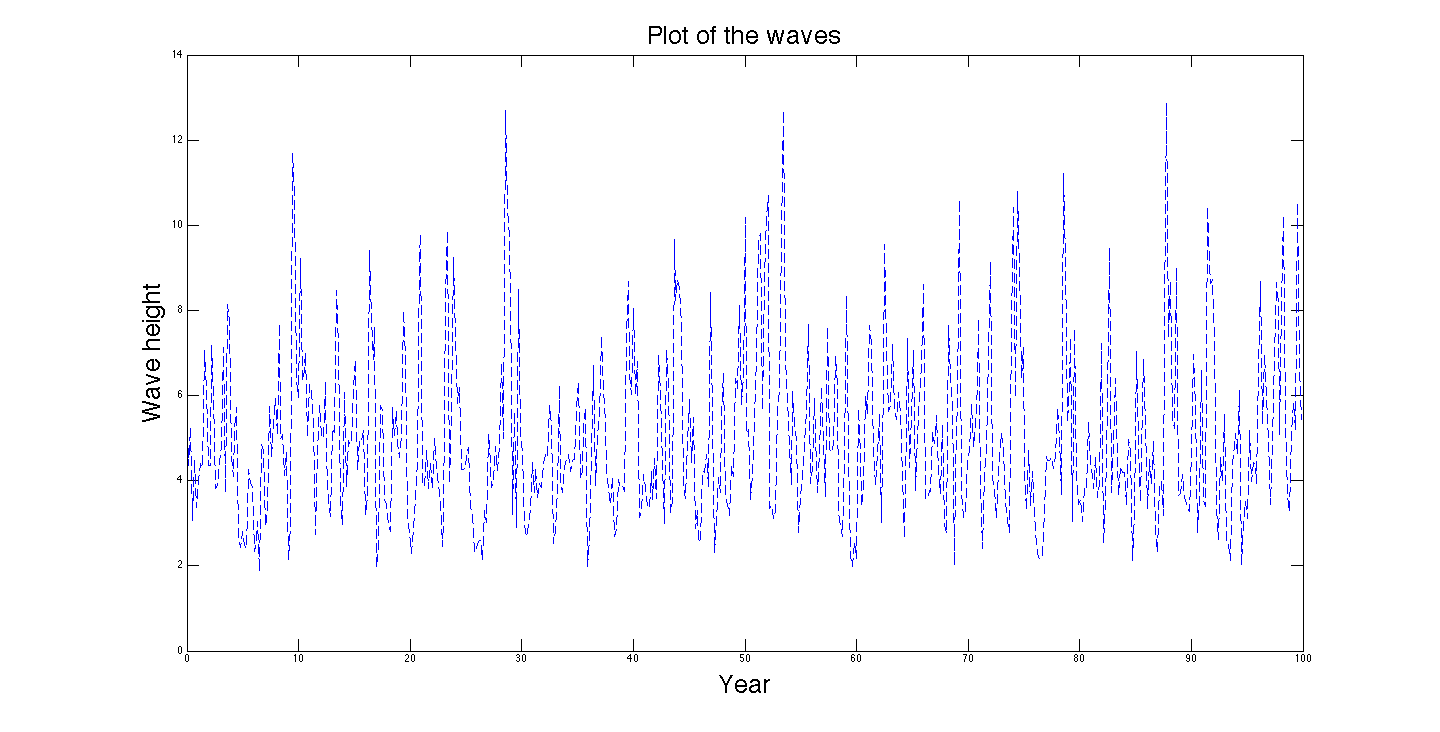
\includegraphics[scale=0.26]{./Figures/waves.png}
\caption{A figure, showing the data of the significant observed wave-heights}
\label{fig:waves}

\end{figure}

To perform a statistical test on the dataset, we use a parametric bootstrap approach. The bootstrap technique evaluates the uncertainty of an unknown distribution or data. The bootstrap replaces the unknown statistic by data-based approximations and analyzes the variation using MC simulation from the approximation. The approximations are done using a \textbf{empirical distribution} (ED) associated with the data and gives equal weights to each observed value. Below we will present a brief description of a general bootstrap method.

\begin{itemize}
\item{For a given statistic y, we replace $\mathbb{P}_0$ by $\hat{\mathbb{P}}_0$.}
\item{Approximation can be done by plugging $\hat{\mathbb{P}}_0$ into the quantity, i.e.
\[ \tau=\tau(\mathbb{P}_0)\approx \hat{\tau}=\tau(\hat{\mathbb{P}}_0) \].}
\item{Uncertainty of $t(y)$ is analyzed by looking at the variation of $\Delta(Y^*)=t(Y^*)-\hat{\tau}$ by drawing repeatedly $Y^*\sim \hat{\mathbb{P}_0}$.}
\end{itemize}

In our case, we have done a parametric bootstrap, where we assume that the data comes from a distribution $\mathbb{P}_0=\mathbb{P}_{\theta_0}\in\{\mathbb{P}_\theta;\theta \in \Theta\}$ belonging to some parametric family. Instead of using the ED, we find an estimate $\hat{\theta}=\hat{\theta}(y)$ of $\theta_0$ from the observations and
\begin{enumerate}
\item{generate new bootstrapped samples $Y_b^*,b\in \{1,2,\dots,B\}$, from $\hat{\mathbb{P}_0}=\mathbb{P}_{\hat{\theta}}$.}
\item{then we form bootstrap estimates $\hat{\theta}(Y_b^*)$ and errors $\Delta_b^*=\hat{\theta}(Y_b^*)-\hat{\theta},b\in\{1,2,\dots,B\}$}.
\end{enumerate}

For this assigment we approximated the data as being that of \textit{Gumpel distributed} data points. In the figure \ref{fig:waveshist} we have plotted the histogram of the atlantic wave-heights, indicating that the data has a a \textit{Gumpel} distribution.

\begin{figure}[H]
\centering
	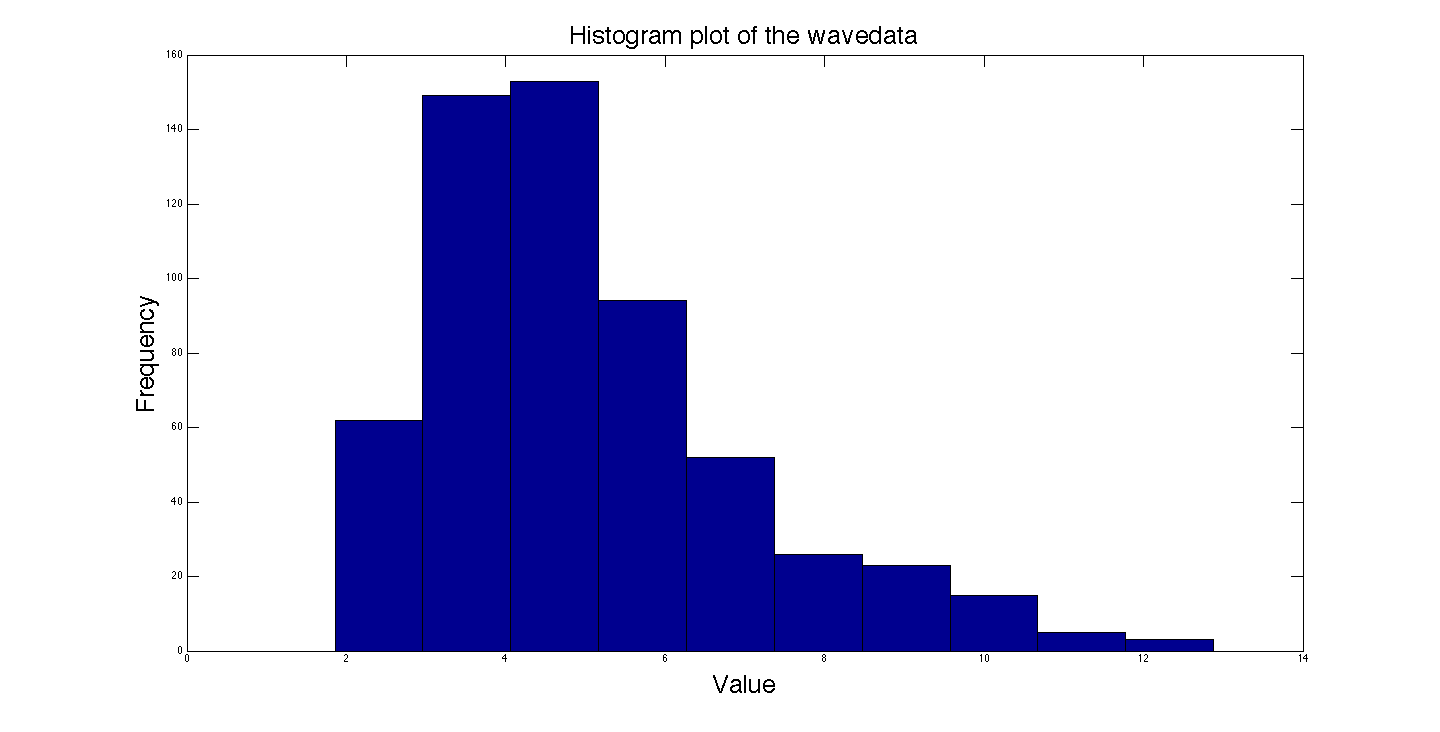
\includegraphics[scale=0.26]{./Figures/waveshist.png}
\caption{A figure, showing the data of the significant observed wave-heightsdata, in \texttt{atlantic.mat}}
\label{fig:waveshist}

\end{figure}
